\documentclass[a4paper,11pt]{refart}

%\usepackage[utf8]{inputenc}
%\usepackage[T1]{fontenc}
\usepackage{fontspec}

\usepackage{microtype}

\usepackage{graphicx}
\usepackage{enumitem}
\setlist{leftmargin=*}
\usepackage{listings}
\lstset{basicstyle=\ttfamily,frame=single,xleftmargin=3em,xrightmargin=3em}
\usepackage{framed}
\usepackage{etoolbox}
\AtBeginEnvironment{leftbar}{\sffamily\small}

\usepackage{hyperref}
\usepackage{longtable}
\usepackage{tabu}
\usepackage{tabularx}

\usepackage[table,dvipsnames,x11names]{xcolor}
\usepackage{booktabs}

\newcommand\AutoCalc{\textsf{AutoratingCalculator}}
\renewcommand\abstractname{Introduction}


%% Custom fonts for showcasing
\newfontfamily{\StarFourK}{Star4000}[Extension = .ttf, Scale=1.2]
\newfontfamily{\StarFourKLg}{Star4000-Large}[Extension = .ttf, Scale=0.9]
\newfontfamily{\StarFourKLgC}{Star4000-Large-Compressed}[Extension = .ttf, Scale=0.9]
\newfontfamily{\StarFourKExt}{Star4000-Extended}[Extension = .ttf, Scale=1.1]
\newfontfamily{\StarFourKSm}{Star4000-Small}[Extension = .ttf, Scale=1.3]
%% ================


\title{WS4 Documentation \& Reference}
\author{Anton Slavin\\\url{anton@slavin.ee}}
\date{Version 0.5\\\today}




\begin{document}

\maketitle

\begin{abstract}
TODO. WS4 is available at \url{https://github.com/tonysln/ws4}.
\end{abstract}

\tableofcontents
\clearpage



\section{Background}

\subsection{WeatherSTAR 4000}

The primary purpose of WeatherStar units is to disseminate weather information for local forecast segments on The Weather Channel. The forecast and observation data – which is compiled from local offices of the National Weather Service (NWS), the Storm Prediction Center (SPC), and The Weather Channel (which began producing in-house forecasts in 2002, replacing the NWS-sourced zone forecasts that were utilized for the STAR's descriptive, regional and extended forecast products) – is received from the vertical blanking interval of the TWC video feed and from data transmitted via satellite; the localized data is then sent to the unit that inserts the data and accompanying programmed graphics over the TWC feed. The WeatherStar systems are typically programmed to cue the local forecast segments and Lower Display Line (LDL) at given times. The units are programmed to feature customized segments known as "flavors," pre-determined segment lengths for each local forecast segment, varying by the time of broadcast, accommodating the inclusion or exclusion of certain products from a segment's product list \cite{WSWiki}. 

The Weather Star 4000 was the first WeatherStar model capable of displaying graphics. First developed in 1988, it was introduced in early 1990. Due to the cost of upgrading to more advanced units including the IntelliStar, the Weather Star 4000 remained in use in some smaller communities as late as 2014, although it was already being gradually phased out in some areas in favor of the more recent models at that time \cite{WSWiki}.

\subsection{Restoration Efforts}

Recently, multiple restoration efforts have started to restore the original WeatherSTAR 4000 units after purchasing them from markets or ...

Some notable cases include ...

...

\subsection{Simulators}

Besides original hardware restoration efforts, multiple simulators have been created by fans and programmers, including:

\begin{itemize}
	\item Taiganet WS4K simulator by Bill et al
	\item WS4000+ online simulator
	\item ...
\end{itemize}

Additionally, fans have been recreating manual scenes using video editing software, such as ...

\subsection{Differences}

In comparison to the simulators and other efforts, WS4 does not aim to be a faithful replication of the original system. Instead, the goal is to create a modern, simple, fast, modular system with very close graphics and layouts, without the excruciating details copied over. The goal is to have a system that would run on a wide variety of hardware with easy setup. Most importantly, it is expected to be very stable in case any of the components fail - such as being able to draw graphics continuously despite not receiving any data for prolonged amount of time and then resuming normal operation.

%\begin{enumerate}
%\item In Notepad, compile the list of group members in your class, using the following format:

%\begin{lstlisting}
%10032,Mary Tan
%10143,Prabakar Murugan
%10033,Tan Beng Huat
%10165,Calvin Ong
%
%10052,Mooi Siok Lan
%10114,Bong Chin Keat
%10432,Joseph Calvin
%10281,Suresh Kappan
%\end{lstlisting}

%  \begin{itemize}[noitemsep]
%  \item Record the \emph{ID} and \emph{name} of a student on each line.
%  \item Use a comma (\texttt{,}) to separate the ID and name on each line.
%  \item Leave an \emph{empty line} between groups.
%  \end{itemize}
  
%\item Save the group list file using \texttt{.txt} or \texttt{.csv} extension, e.g.\\\texttt{DIT1234-Apr2013-groups.txt}.
%
%\medskip
%
%\begin{leftbar}
%You may also prepare the group list in Excel. List the IDs in column A and the IDs in column B. Save the file as a Comma separated values file (CSV). In the Export Filter Settings, set text delimiter to blank, and field separator to comma (\texttt{,}).
%\end{leftbar}
%
%\end{enumerate}


\newpage
\section{Features}

\subsection{Available Screens ("Products")}

\subsubsection*{Current Conditions}

\begin{figure}[ht!]\centering
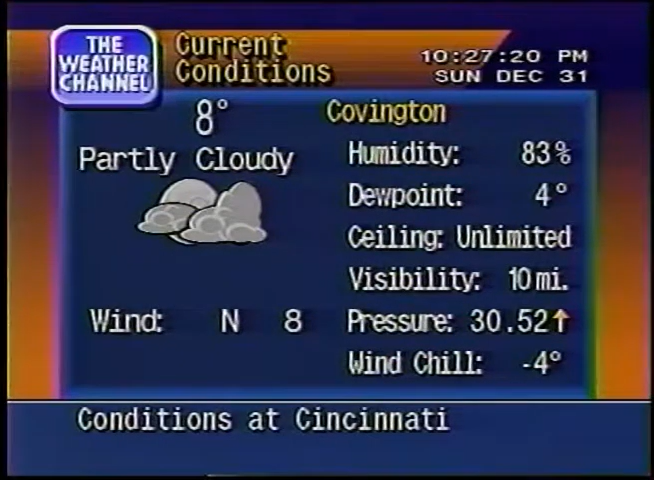
\includegraphics[width=\textwidth]{img/current-conditions.png}
%\caption{Current Conditions}\label{fig:curcond}
\end{figure}

The Current Conditions Page is the first page that displays during the Local Forecast. It shows in every Local Forecast. It is driven by the primary and alternate sites of the STAR 4000. It displays the current weather conditions for that location. It is not forecast data, nor is it related to where the forecast comes from \cite{WS4KProdGde}.

\subsubsection*{Latest Observations}

\begin{figure}[ht!]\centering
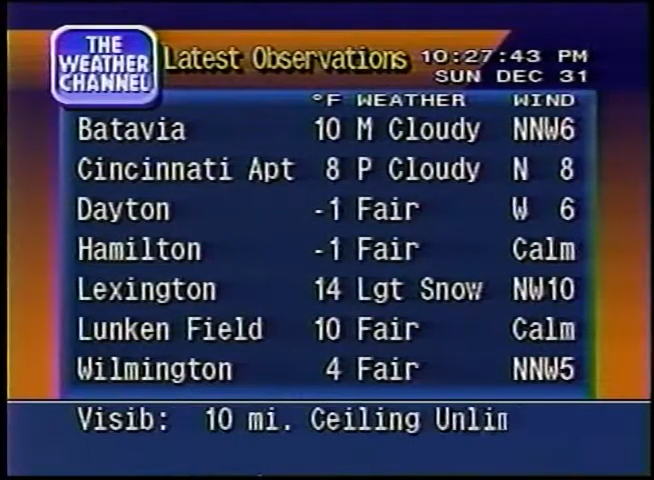
\includegraphics[width=\textwidth]{img/latest-observ.png}
%\caption{Latest Observations}\label{fig:latestobs}
\end{figure}


The Local Observations Page is the second page that usually displays during the Local Forecast. It shows in every Local Forecast. It is driven by the seven closest weather observation sites to the STAR 4000. It displays the current weather conditions for those locations. It is not forecast data \cite{WS4KProdGde}.

\subsubsection*{Regional Observations Map}

\begin{figure}[ht!]\centering
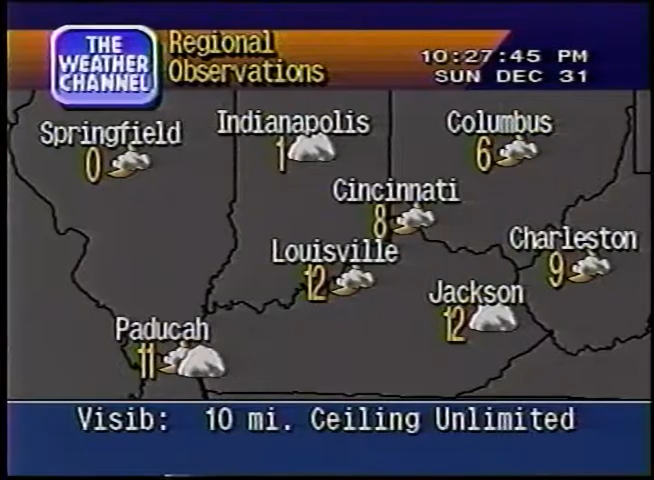
\includegraphics[width=\textwidth]{img/reg-observ.png}
%\caption{Regional Observations}\label{fig:regobs}
\end{figure}

The Regional Observations Map only displays once an hour (usually the forecast :58 minutes after the hour) and is the fourth page that displays during the Local Forecast in that flavor. It is driven by the weather observation sites of the largest cities in the region around the STAR that will fit on the map. It displays the current weather conditions for those locations. It is not forecast data \cite{WS4KProdGde}.

\subsubsection*{36-Hour Forecast Pages}

\begin{figure}[ht!]\centering
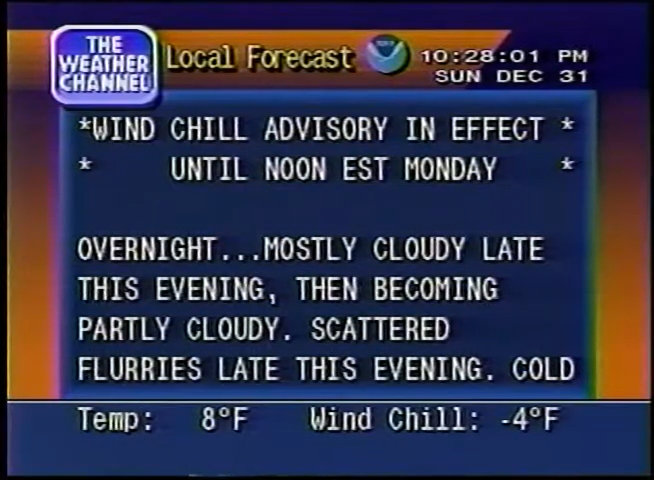
\includegraphics[width=\textwidth]{img/36hour.png}
%\caption{36-Hour Forecast}\label{fig:36hour}
\end{figure}

The three 36-Hour Forecast pages display near the middle of The Local Forecast. It is driven by National Weather Service (NWS) zone, not primary or alternate site, and is considered narrative data. The forecast is generated by the NWS specifically for each county in the U.S. The forecast is not generated by The Weather Channel.

The first period of the time interval switches during the main update times. In the morning, after about 5 am local time, a 36-hour forecast should begin with the time period “This Morning” or “Today”, not “Tonight”. In the evening, after about 5 pm local time, the 36-hour forecast should begin with the period “This evening”, “Overnight”, or “Tonight”, not “This Afternoon”. If these time periods are still old, there may be a problem with the narrative data \cite{WS4KProdGde}.

\subsubsection*{Regional Forecast Map}

\begin{figure}[ht!]\centering
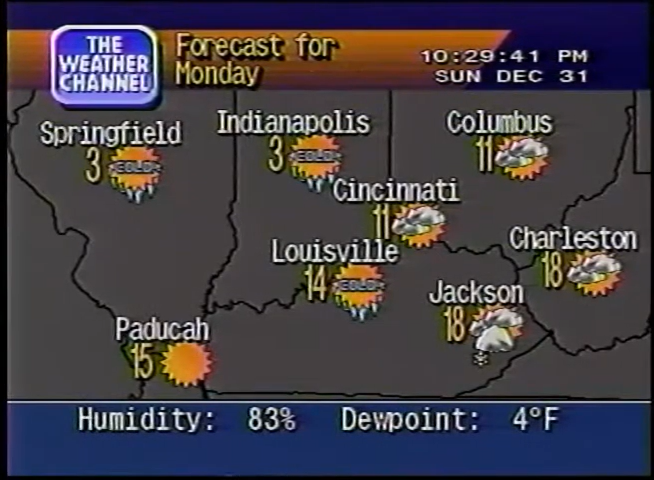
\includegraphics[width=\textwidth]{img/reg-forc.png}
%\caption{Regional Forecast}\label{fig:regforc}
\end{figure}

The Regional Forecast Map only displays once an hour (usually the forecast :58 minutes after the hour). It displays the forecast weather condition (icon) and high temperature for those locations in the region around the STAR on a map. It is forecast data \cite{WS4KProdGde}.

\subsubsection*{Extended Forecast}

\begin{figure}[ht!]\centering
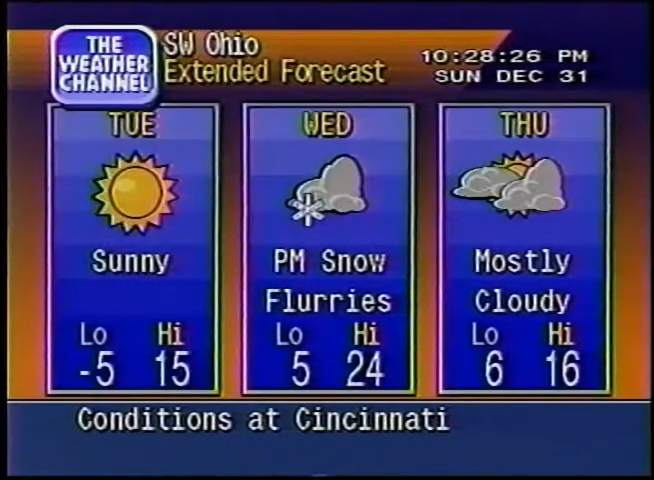
\includegraphics[width=\textwidth]{img/ext-forc.png}
%\caption{Extended Forecast}\label{fig:extforc}
\end{figure}

The Extended Forecast displays in every Local Forecast and usually displays after the 36-Hour Forecast or Regional Forecast Map during the Local Forecast. The data (FE data) is driven by extended weather forecasts made TWC meteorologists for areas across the country. It displays the forecast weather condition (icon), low and high temperature for those locations for a three day period. It is forecast data.

The FE data for these pages is sent at 5 am to adjust the days, and then updated 3 more times during the day. The 5 am update adjusts the day one day forward. For example, before 5 am on Tuesday, the 3 to 5 days will display as “Wed”, “Thu”, and “Fri”. After 5 am on Tuesday, the days will display as “Thu”, “Fri”, and “Sat”. Those days will display until 5 am Wednesday \cite{WS4KProdGde}.

\subsubsection*{Almanac}

\begin{figure}[ht!]\centering
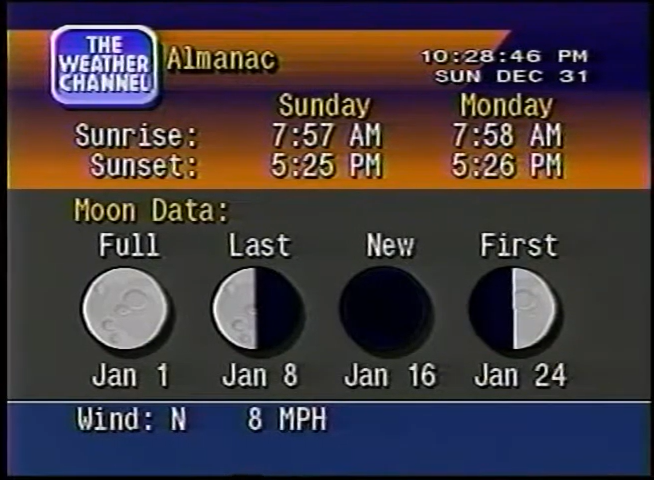
\includegraphics[width=\textwidth]{img/almanac.png}
%\caption{Almanac}\label{fig:almanac}
\end{figure}

The Almanac page displays once an hour (usually the forecast :58 minutes after the hour). The data is calculated on the STAR host based on the latitude/longitude of the climate station assigned to the Weather Display Area (WDA) the STAR is assigned. The data is then sent to the STARs a couple of times a day. It displays the sunrise/sunset times for the next 2 days. It also displays the next 4 moon phases and the dates of each phase.

The times are based on the local tie of the headend and follow the daylight savings time (DST) rules of the time zone and local laws of the headend (the states of Arizona and Hawaii, Puerto Rico, the Virgin Islands, and some counties in Indiana do not observe DST). The sunrise/sunset data is updated at midnight, local time \cite{WS4KProdGde}.

\subsubsection*{Air Quality}
...

\subsubsection*{Marine Forecast}
...

\subsubsection*{Tides}
...

\subsubsection*{Travel Forecast}
...

\subsubsection*{Airport}
...



\subsection{Locations}

Ideally all over the world... Highlights USA, Europe, Asia, Antarctica...

For USA, great API from the NWS and NOAA.

Other areas harder...

\subsection{Music}

Music from non-licensed sources, so not shared but easily supported. Some artists list for free (Patrick O'Hearn), also on YouTube...

Narration not supported.


\begin{enumerate}
\item Launch the \AutoCalc\ tool by double-clicking on its icon in Windows Explorer.
\item From the menu bar, select File>Import... or press Ctrl+I.
\item Select a \emph{group list file} (\texttt{*.txt, *.csv}) to import from, e.g.\\\texttt{DIT1234-Apr2013-groups.txt}.
\item \AutoCalc\ will then ask you for a \emph{new} file name to save the new score list as (\texttt{*.xml}), e.g.~\texttt{DIT1234-Apr2013-Assgn1.xml}.


\medskip

\begin{leftbar}
Make sure the \texttt{.xml} score filename selected does not already exist. Otherwise the existing score file \textbf{may be overwritten without warning}!
\end{leftbar}

\medskip

\item \AutoCalc\ imports the group lists and displays the student IDs and names in the main panel (Figure~\ref{fig:grouplist}).

\begin{figure}[hbt!]\centering
%\includegraphics[width=\textwidth]{grouplist}
\caption{Imported group list}\label{fig:grouplist}
\end{figure}
\end{enumerate}



\newpage
\section{Style Details}

What follows is a detailed description of all elements used in drawing screens for WS4. This can be used as a reference point for future builds, forks, updates and other similar projects. The goal is to collect the most exact and latest information and keep updating it here as a main reference point.

Starting off with simpler things like colors and fonts, this section will end with descriptions of how the layout is drawn in WS4, what are the components that go into it and in which order.

\subsection{Colors}

The following colors are defined for use in the whole WS4 application, for all screens. Each color is represented in hexadecimal and RGB forms, and contains examples on where the color is most often used in the interface.

\begin{centering}
\begin{longtabu}{cccc}
  \textbf{Color}  & \textbf{Hex} & \textbf{RGB} & \textbf{Usage} \\
  \midrule
  \textcolor[rgb]{0.14, 0.14, 0.14}{\rule{.1\textwidth}{12pt}}  & \texttt{\#0e0e0e}    & \texttt{(14,14,14)} & Shadows \\
  \textcolor[rgb]{0.20, 0.20, 0.20}{\rule{.1\textwidth}{12pt}}  & \texttt{\#141414}    & \texttt{(20,20,20)} & Backdrops \\
  \textcolor[cmyk]{0, 0, 0, 0.16}{\rule{.1\textwidth}{12pt}}  & \texttt{\#d7d7d7}    & \texttt{(215,215,215)} & White Text \\
  \textcolor[cmyk]{0, 0, 0, 0.3137}{\rule{.1\textwidth}{12pt}}  & \texttt{\#afafaf}    & \texttt{(175,175,175)} & LDL Gray Line \\
  \textcolor[cmyk]{0, 0, 0, 0.7608}{\rule{.1\textwidth}{12pt}}  & \texttt{\#3d3d3d}    & \texttt{(61, 61, 61)} & Almanac BG \\
  \textcolor[cmyk]{0, 0.0976, 1, 0.1961}{\rule{.1\textwidth}{12pt}}  & \texttt{\#cdb900}    & \texttt{(205,185,0)} & Yellow Text \\
  \textcolor[cmyk]{0.47, 0.44, 0, 0.04}{\rule{.1\textwidth}{12pt}}  & \texttt{\#828af5}    & \texttt{(130,138,245)} & EF Panel Border \\
  \textcolor[cmyk]{0.68, 0.89, 0, 0.66}{\rule{.1\textwidth}{12pt}}  & \texttt{\#1c0a57}    & \texttt{(28,10,87)} & Main Background \\
  \textcolor[cmyk]{0.6875, 0.5536, 0, 0.5608}{\rule{.1\textwidth}{12pt}}  & \texttt{\#233270}    & \texttt{(35,50,112)} & LDL Background \\
  \textcolor[cmyk]{0, 0.7407, 0.8889, 0.4706}{\rule{.1\textwidth}{12pt}}  & \texttt{\#87230f}    & \texttt{(135,35,15)} & LDL Emergency BG \\
  \textcolor[cmyk]{0.4321, 0.7778, 0, 0.6824}{\rule{.1\textwidth}{12pt}}  & \texttt{\#2e1251}    & \texttt{(46,18,81)} & Main Gradient Bot \\
  \textcolor[cmyk]{0, 0.5156, 0.9896, 0.2471}{\rule{.1\textwidth}{12pt}}  & \texttt{\#c05d02}    & \texttt{(192,93,2)} & Main Gradient Top \\
  \textcolor[cmyk]{0, 0.5333, 1, 0.2353}{\rule{.1\textwidth}{12pt}}  & \texttt{\#c35b00}    & \texttt{(195,91,0)} & Top Bar BG 1 \\
  \textcolor[cmyk]{0, 0.5393, 1, 0.3020}{\rule{.1\textwidth}{12pt}}  & \texttt{\#b25200}    & \texttt{(178,82,0)} & Top Bar BG 2 \\
  \textcolor[cmyk]{0, 0.5223, 0.8790, 0.3843}{\rule{.1\textwidth}{12pt}}  & \texttt{\#9d4b13}    & \texttt{(157,75,19)} & Top Bar BG 3 \\
  \textcolor[cmyk]{0, 0.5352, 0.8169, 0.4431}{\rule{.1\textwidth}{12pt}}  & \texttt{\#8e421a}    & \texttt{(142,66,26)} & Top Bar BG 4 \\
  \textcolor[cmyk]{0, 0.5447, 0.7073, 0.5176}{\rule{.1\textwidth}{12pt}}  & \texttt{\#7b3824}    & \texttt{(123,56,36)} & Top Bar BG 5 \\
  \textcolor[cmyk]{0, 0.5619, 0.5619, 0.5882}{\rule{.1\textwidth}{12pt}}  & \texttt{\#692e2e}    & \texttt{(105,46,46)} & Top Bar BG 6 \\
  \textcolor[cmyk]{0, 0.5281, 0.3034, 0.6510}{\rule{.1\textwidth}{12pt}}  & \texttt{\#592a3e}    & \texttt{(89,42,62)} & Top Bar BG 7 \\
  \textcolor[cmyk]{0, 0.5211, 0.0986, 0.7216}{\rule{.1\textwidth}{12pt}}  & \texttt{\#472240}    & \texttt{(71,34,64)} & Top Bar BG 8 \\
  \textcolor[cmyk]{0, 0.5200, 0.6800, 0.5098}{\rule{.1\textwidth}{12pt}}  & \texttt{\#7d3c28}    & \texttt{(125,60,40)} & Almanac Top BG \\
  \textcolor[cmyk]{0.7865, 0.5393, 0, 0.3020}{\rule{.1\textwidth}{12pt}}  & \texttt{\#2652b2}    & \texttt{(38,82,178)} & Blue Pane Layer 1 \\
  \textcolor[cmyk]{0.7730, 0.5399, 0, 0.3608}{\rule{.1\textwidth}{12pt}}  & \texttt{\#254ba3}    & \texttt{(37,75,163)} & Blue Pane Layer 2 \\
  \textcolor[cmyk]{0.7566, 0.5395, 0, 0.4039}{\rule{.1\textwidth}{12pt}}  & \texttt{\#254698}    & \texttt{(37,70,152)} & Blue Pane Layer 3 \\
  \textcolor[cmyk]{0.7429, 0.5429, 0, 0.4510}{\rule{.1\textwidth}{12pt}}  & \texttt{\#24408c}    & \texttt{(36,64,140)} & Blue Pane Layer 4 \\
  \textcolor[cmyk]{0.7266, 0.5469, 0, 0.4980}{\rule{.1\textwidth}{12pt}}  & \texttt{\#233a80}    & \texttt{(35, 58, 128)} & Blue Pane Layer 5 \\
  \textcolor[cmyk]{0.7069, 0.5517, 0, 0.5451}{\rule{.1\textwidth}{12pt}}  & \texttt{\#223474}    & \texttt{(34,52,116)} & Blue Pane Layer 6 \\
  \textcolor[cmyk]{0.6762, 0.5524, 0, 0.5882}{\rule{.1\textwidth}{12pt}}  & \texttt{\#222f69}    & \texttt{(34,47,105)} & Blue Pane Layer 7 \\
  \textcolor[cmyk]{0.6563, 0.5521, 0, 0.6235}{\rule{.1\textwidth}{12pt}}  & \texttt{\#212b60}    & \texttt{(33,43,96)} & Blue Pane Layer 8 \\
  \textcolor[cmyk]{0.6333, 0.5556, 0, 0.6471}{\rule{.1\textwidth}{12pt}}  & \texttt{\#21285a}    & \texttt{(33,40,90)} & Blue Pane Layer 9 \\
  \textcolor[cmyk]{0.5743, 0.5495, 0, 0.2078}{\rule{.1\textwidth}{12pt}}  & \texttt{\#565bca}    & \texttt{(86,91,202)} & EF Panel Seg 1 \\
  \textcolor[cmyk]{0.6733, 0.6139, 0, 0.2078}{\rule{.1\textwidth}{12pt}}  & \texttt{\#424eca}    & \texttt{(66,78,202)} & EF Panel Seg 2 \\
  \textcolor[cmyk]{0.7822, 0.6733, 0, 0.2078}{\rule{.1\textwidth}{12pt}}  & \texttt{\#2c42ca}    & \texttt{(44,66,202)} & EF Panel Seg 3 \\
  \textcolor[cmyk]{0.8168, 0.7178, 0, 0.2078}{\rule{.1\textwidth}{12pt}}  & \texttt{\#2539ca}    & \texttt{(37,57,202)} & EF Panel Seg 4 \\
  \textcolor[cmyk]{0.9554, 0.7574, 0, 0.2078}{\rule{.1\textwidth}{12pt}}  & \texttt{\#0931ca}    & \texttt{(9,49,202)} & EF Panel Seg 5 \\
  \textcolor[cmyk]{1, 0.8030, 0, 0.2039}{\rule{.1\textwidth}{12pt}}  & \texttt{\#0028cb}    & \texttt{(0,40,203)} & EF Panel Seg 6 \\
  \textcolor[cmyk]{1, 0.8227, 0, 0.2039}{\rule{.1\textwidth}{12pt}}  & \texttt{\#0024cb}    & \texttt{(0,36,203)} & EF Panel Seg 7 \\
  \textcolor[cmyk]{1, 0.8325, 0, 0.2039}{\rule{.1\textwidth}{12pt}}  & \texttt{\#0022cb}    & \texttt{(0,34,203)} & EF Panel Seg 8 \\
\end{longtabu}
\end{centering}

The colors were chosen by looking through hundreds of reference videos, photos, and simulator screenshots.

More detailed information on the usage of colors can be found in upcoming sections for layout ...

\subsection{Fonts}

Double-click on the name of a student in the list to display the peer review score entry window.

\begin{table}[h]
\centering
\begin{tabular}{ll}
  \textbf{Font}  & \textbf{Usage} \\
  \midrule
  {\StarFourK Star4000} & Most Text Labels \\
  {\StarFourKLg Star4000 Large} & EF Temp Values \\
  {\StarFourKLgC Star4000 Large Compressed} & Map Temp Values \\
  {\StarFourKExt Star4000 Extended} & CC Left-Side Info \\
  {\StarFourKSm Star4000 Small} & Clock, LO Headers
\end{tabular}
\end{table}

The fonts have been acquired from TWC Classics courtesy of Nick Smith \cite{TWCClassicsDownloads}.

\subsection{Icons}

You can also load the peer ratings entry window of a student by keying in the ID number in the search box, and then click on the Search button.

\subsection{Layout}

Some main elements present in screens ...

\begin{enumerate}
\item Main background (single color)
\item Main gradient ...
\item Top bar ...
\item Center panel ...
\item LDL (with two lines on top) over all content ...
\end{enumerate}

Then any icons that have to be drawn and animated ...

Text on top of main elements ...

\begin{enumerate}
\item Date and time
\item Title of screen
\item Static text
\item Dynamic text
\item LDL overlay text
\end{enumerate}

\subsection{Computing Autorated Scores}
\begin{enumerate}
\item When peer ratings of all students in a group has been entered and committed, click on the Compute Weights and Scores button. The computed weights and scores will be saved to file immediately.
\item Click on the Group Overview tab to see autorated weights and scores for each student in the group.

\begin{figure}[hbt!]
%\includegraphics[width=\textwidth]{groupoverview}
\caption{Autorated Weights and Scores of Group Members}
\end{figure}

\end{enumerate}



\newpage
\section{Structure}

\subsection{Storing Assets}

\subsection{Drawing Graphics}

\subsection{Fetching Data}


You may open an existing assignment score file (\texttt{*.xml}) to inspect scores, as well as to change settings and recalculate scores.
\begin{enumerate}
\item To open an existing score file, access the menu item File>Open\ldots or press Ctrl+O.
\item Locate and select the \texttt{*.xml} file to open.
\end{enumerate}



\newpage
\section{Implementation}
The autorated scores can be exported for further processing in Excel.
\begin{enumerate}
\item Select File>Export\ldots from the menu, or Ctrl+E.
\item Select a file name to save the exported data in. The file will be saved with a \texttt{.csv} extension. %\includegraphics[height=1em]{csv}
\item In Windows Explorer, locate the \texttt{.csv} file and double-click on it to open it in Excel.
\item If warning messages are displayed, keep on clicking OK or Yes to ignore them.
\item When the data is displayed, you may save the file as an \texttt{.xlsx} or \texttt{.xsl} Excel file, and continue processing it.

\begin{figure}[hbt!]
%\includegraphics[width=\textwidth]{excel}
\caption{Exported data in Excel}
\end{figure}

\end{enumerate}


\newpage
\bibliographystyle{plain}
\bibliography{refs.bib}
\end{document}